\begin{figure}[tbp]
\centering
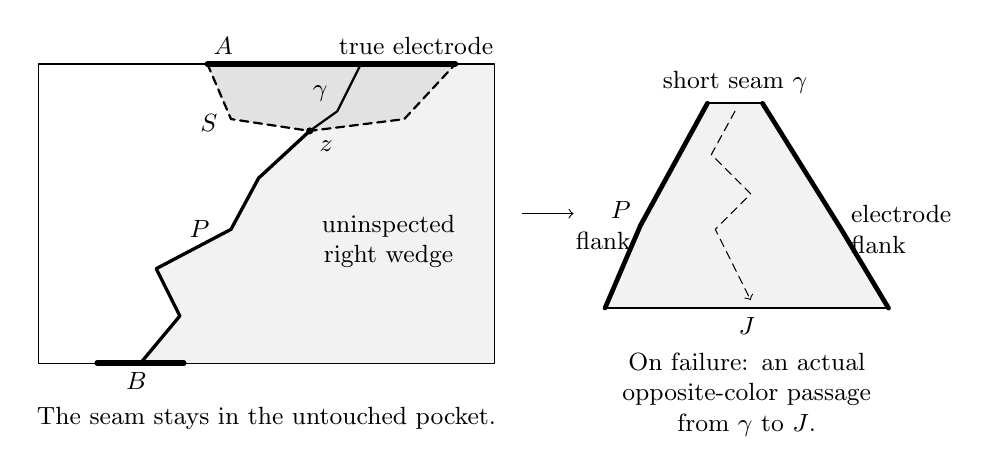
\begin{tikzpicture}[x=1cm,y=1cm,font=\small,line cap=round,line join=round]
  \path[fill=gray!10] (1.3,0) -- (1.8,.6) -- (1.5,1.2) -- (2.45,1.7)
    -- (2.8,2.35) -- (3.45,2.95) -- (4.1,3.8) -- (5.8,3.8) -- (5.8,0) -- cycle;
  \path[fill=gray!23] (2.15,3.8) -- (2.45,3.1) -- (3.45,2.95) -- (4.65,3.1) -- (5.3,3.8) -- cycle;
  \draw (0,0) rectangle (5.8,3.8);
  \draw[line width=2pt] (2.15,3.8) -- (5.3,3.8);
  \draw[line width=2pt] (.75,0) -- (1.85,0);
  \draw[densely dashed,thick] (2.15,3.8) -- (2.45,3.1) -- (3.45,2.95) -- (4.65,3.1) -- (5.3,3.8);
  \draw[line width=1.2pt] (1.3,0) -- (1.8,.6) -- (1.5,1.2) -- (2.45,1.7)
    -- (2.8,2.35) -- (3.45,2.95);
  \draw[thick] (3.45,2.95) -- (3.8,3.2) -- (4.1,3.8);
  \fill (3.45,2.95) circle (.045);
  \node[below right] at (3.45,2.95) {$z$};
  \node[left] at (2.3,1.7) {$P$};
  \node[above] at (2.35,3.8) {$A$};
  \node[below] at (1.25,0) {$B$};
  \node[left] at (2.4,3.05) {$S$};
  \node[left] at (3.8,3.42) {$\gamma$};
  \node[align=center] at (4.45,1.55) {uninspected\\right wedge};
  \node[above] at (4.8,3.8) {true electrode};
  \node[align=center] at (2.9,-.7) {The seam stays in the untouched pocket.};
  \draw[->] (6.15,1.9) -- (6.8,1.9);
  \path[fill=gray!10] (7.2,.7) -- (7.65,1.75) -- (8.5,3.3) -- (9.2,3.3)
    -- (10.2,1.7) -- (10.8,.7) -- cycle;
  \draw[line width=1.7pt] (7.2,.7) -- (7.65,1.75) -- (8.5,3.3);
  \draw[line width=1.7pt] (9.2,3.3) -- (10.2,1.7) -- (10.8,.7);
  \draw[thick] (8.5,3.3) -- (9.2,3.3);
  \draw[thick] (7.2,.7) -- (10.8,.7);
  \draw[densely dashed,->] (8.85,3.2) -- (8.55,2.65) -- (9.05,2.15) -- (8.6,1.7) -- (9.05,.8);
  \node[above] at (8.85,3.3) {short seam $\gamma$};
  \node[below] at (9,.7) {$J$};
  \node[left,align=right] at (7.65,1.75) {$P$\\flank};
  \node[right,align=left] at (10.2,1.7) {electrode\\flank};
  \node[align=center,text width=4.8cm] at (9,-.4)
    {On failure: an actual\\opposite-color passage\\from $\gamma$ to $J$.};
\end{tikzpicture}
\caption{Extending a moving electrode. Left: an actual extremal path $P$ first hits the inset cut $S$ at $z$; the small seam $\gamma$ reaches the true electrode through the untouched pocket. The tail after the last right-boundary hit, the seam, and the right outer boundary bound the protected wedge. Right: the subdisk between the seam and a farther cut $J$, drawn in abstract disk coordinates. Both flanks are wired in the tested color. Failure of their connection is an actual opposite-color hard passage with ties confined to its ends. The wedge is chosen from measured information; the future failure event is not used to condition its law.}
\label{fig:short-seam}
\end{figure}
